\documentclass[preprint,number]{elsarticle}

\usepackage{amsmath,amssymb}
\usepackage{graphicx}
\graphicspath{{./}{../figs/}{figs/}}
\usepackage{booktabs}
\usepackage{url}
\setlength{\emergencystretch}{1em}

\journal{Neurocomputing}

\makeatletter
\def\ps@pprintTitle{%
  \let\@oddhead\@empty
  \let\@evenhead\@empty
  \def\@oddfoot{\hbox to \textwidth{\footnotesize\itshape
    Preprint submitted to \@journal\hfill\@date}}%
  \let\@evenfoot\@oddfoot}
\makeatother

\newcommand{\rhosp}{\ensuremath{\rho}}
% Any text still waiting for the round-2 second-backbone run is wrapped in \pending.
% tools/audit_paper2_v2.py fails while the word PENDING appears in the PDF.
\newcommand{\pending}[1]{\textbf{[PENDING: #1]}}
\newcommand{\supp}[1]{Supplementary Section~S#1}
% \seedlabel{key}{rule} / \seeddetail{key}{rule}: three-seed labels from aggregate.json
% (generated; a label still waiting for a seed expands to \pending).
% Generated by tools/make_paper2_extra_tables.py -- do not edit by hand.
\providecommand{\seedlabel}[2]{\csname seedlabel-#1-#2\endcsname}
\providecommand{\seeddetail}[2]{\csname seeddetail-#1-#2\endcsname}
\expandafter\def\csname seedlabel-qwen25vl3b-R1\endcsname{is not established}
\expandafter\def\csname seeddetail-qwen25vl3b-R1\endcsname{seed 42: intermediate; 43: replicates; 44: intermediate}
\expandafter\def\csname seedlabel-qwen25vl3b-R2_E\endcsname{is not established}
\expandafter\def\csname seeddetail-qwen25vl3b-R2_E\endcsname{seed 42: intermediate; 43: untestable; 44: intermediate}
\expandafter\def\csname seedlabel-qwen25vl3b-R2_T\endcsname{is not established}
\expandafter\def\csname seeddetail-qwen25vl3b-R2_T\endcsname{seed 42: intermediate; 43: intermediate; 44: intermediate}
\expandafter\def\csname seedlabel-qwen25vl3b-R3\endcsname{holds at all three seeds}
\expandafter\def\csname seeddetail-qwen25vl3b-R3\endcsname{seed 42: replicates; 43: replicates; 44: replicates}
\expandafter\def\csname seedlabel-qwen25vl3b-R4\endcsname{holds at two of three seeds}
\expandafter\def\csname seeddetail-qwen25vl3b-R4\endcsname{seed 42: untestable; 43: replicates; 44: replicates}
\expandafter\def\csname seedlabel-internvl3_2b-R1\endcsname{holds at two of three seeds}
\expandafter\def\csname seeddetail-internvl3_2b-R1\endcsname{seed 42: intermediate; 43: replicates; 44: replicates}
\expandafter\def\csname seedlabel-internvl3_2b-R2_E\endcsname{is not established}
\expandafter\def\csname seeddetail-internvl3_2b-R2_E\endcsname{seed 42: untestable; 43: untestable; 44: replicates}
\expandafter\def\csname seedlabel-internvl3_2b-R2_T\endcsname{holds at two of three seeds}
\expandafter\def\csname seeddetail-internvl3_2b-R2_T\endcsname{seed 42: replicates; 43: untestable; 44: replicates}
\expandafter\def\csname seedlabel-internvl3_2b-R3\endcsname{fails across seeds}
\expandafter\def\csname seeddetail-internvl3_2b-R3\endcsname{seed 42: fails; 43: fails; 44: fails}
\expandafter\def\csname seedlabel-internvl3_2b-R4\endcsname{holds at all three seeds}
\expandafter\def\csname seeddetail-internvl3_2b-R4\endcsname{seed 42: replicates; 43: replicates; 44: replicates}
\expandafter\def\csname seedlabel-pixtral_12b-R1\endcsname{holds at all three seeds}
\expandafter\def\csname seeddetail-pixtral_12b-R1\endcsname{seed 42: replicates; 43: replicates; 44: replicates}
\expandafter\def\csname seedlabel-pixtral_12b-R2_E\endcsname{holds at two of three seeds}
\expandafter\def\csname seeddetail-pixtral_12b-R2_E\endcsname{seed 42: intermediate; 43: replicates; 44: replicates}
\expandafter\def\csname seedlabel-pixtral_12b-R2_T\endcsname{is not established}
\expandafter\def\csname seeddetail-pixtral_12b-R2_T\endcsname{seed 42: untestable; 43: intermediate; 44: untestable}
\expandafter\def\csname seedlabel-pixtral_12b-R3\endcsname{is seed-dependent}
\expandafter\def\csname seeddetail-pixtral_12b-R3\endcsname{seed 42: replicates; 43: fails; 44: replicates}
\expandafter\def\csname seedlabel-pixtral_12b-R4\endcsname{holds at two of three seeds}
\expandafter\def\csname seeddetail-pixtral_12b-R4\endcsname{seed 42: untestable; 43: replicates; 44: replicates}
\expandafter\def\csname seedlabel-idefics3_8b-R1\endcsname{is not established}
\expandafter\def\csname seeddetail-idefics3_8b-R1\endcsname{seed 42: untestable; 43: replicates; 44: intermediate}
\expandafter\def\csname seedlabel-idefics3_8b-R2_E\endcsname{is not established}
\expandafter\def\csname seeddetail-idefics3_8b-R2_E\endcsname{seed 42: intermediate; 43: intermediate; 44: untestable}
\expandafter\def\csname seedlabel-idefics3_8b-R2_T\endcsname{is not established}
\expandafter\def\csname seeddetail-idefics3_8b-R2_T\endcsname{seed 42: intermediate; 43: intermediate; 44: intermediate}
\expandafter\def\csname seedlabel-idefics3_8b-R3\endcsname{holds at two of three seeds}
\expandafter\def\csname seeddetail-idefics3_8b-R3\endcsname{seed 42: intermediate; 43: replicates; 44: replicates}
\expandafter\def\csname seedlabel-idefics3_8b-R4\endcsname{is not established}
\expandafter\def\csname seeddetail-idefics3_8b-R4\endcsname{seed 42: untestable; 43: replicates; 44: intermediate}
\expandafter\def\csname seedlabel-gemma3_12b-R1\endcsname{is seed-dependent}
\expandafter\def\csname seeddetail-gemma3_12b-R1\endcsname{seed 42: fails; 43: intermediate; 44: replicates}
\expandafter\def\csname seedlabel-gemma3_12b-R2_E\endcsname{is not established}
\expandafter\def\csname seeddetail-gemma3_12b-R2_E\endcsname{seed 42: untestable; 43: untestable; 44: untestable}
\expandafter\def\csname seedlabel-gemma3_12b-R2_T\endcsname{is not established}
\expandafter\def\csname seeddetail-gemma3_12b-R2_T\endcsname{seed 42: intermediate; 43: intermediate; 44: intermediate}
\expandafter\def\csname seedlabel-gemma3_12b-R3\endcsname{fails across seeds}
\expandafter\def\csname seeddetail-gemma3_12b-R3\endcsname{seed 42: fails; 43: fails; 44: fails}
\expandafter\def\csname seedlabel-gemma3_12b-R4\endcsname{holds at all three seeds}
\expandafter\def\csname seeddetail-gemma3_12b-R4\endcsname{seed 42: replicates; 43: replicates; 44: replicates}
\expandafter\def\csname seedlabel-smol-R1\endcsname{is not established}
\expandafter\def\csname seeddetail-smol-R1\endcsname{seed 42: intermediate; 43: intermediate; 44: untestable}
\expandafter\def\csname seedlabel-smol-R2_E\endcsname{is not established}
\expandafter\def\csname seeddetail-smol-R2_E\endcsname{seed 42: untestable; 43: untestable; 44: untestable}
\expandafter\def\csname seedlabel-smol-R2_T\endcsname{is not established}
\expandafter\def\csname seeddetail-smol-R2_T\endcsname{seed 42: intermediate; 43: untestable; 44: untestable}
\expandafter\def\csname seedlabel-smol-R3\endcsname{fails across seeds}
\expandafter\def\csname seeddetail-smol-R3\endcsname{seed 42: fails; 43: fails; 44: fails}
\expandafter\def\csname seedlabel-smol-R4\endcsname{is not established}
\expandafter\def\csname seeddetail-smol-R4\endcsname{seed 42: intermediate; 43: intermediate; 44: intermediate}


\begin{document}

\begin{frontmatter}

\title{Order without Magnitude: Single-Unit Fine-Tuning Can Make
       Vision--Language Models Rank Motion but Ignore the Requested Unit}

\author[qdu]{Jun Ji\fnref{orcid1}}
\ead{junji@qdu.edu.cn}
\author[hkust]{Bowen Tan\fnref{orcid2}}
\ead{btanab@connect.ust.hk}
\author[ruc]{Yizhou Zhao\fnref{orcid6}}
\ead{yizhou-zhao@ruc.edu.cn}
\author[qdu]{Yi Li\fnref{orcid3}}
\ead{ly2005@qdu.edu.cn}
\author[qdu]{Xiaolei Zhang\fnref{orcid4}}
\ead{zhangxiaolei@qdu.edu.cn}
\author[qdu]{Yi Sui\corref{cor1}\fnref{orcid5}}
\ead{suiyi@qdu.edu.cn}
\cortext[cor1]{Corresponding author.}
\fntext[orcid1]{ORCID: 0000-0003-3194-2183.}
\fntext[orcid2]{ORCID: 0009-0007-0554-9261.}
\fntext[orcid6]{ORCID: 0009-0004-7515-6322.}
\fntext[orcid3]{ORCID: 0000-0002-4185-3152.}
\fntext[orcid4]{ORCID: 0000-0002-0122-4554.}
\fntext[orcid5]{ORCID: 0009-0001-8081-5183.}
\address[qdu]{College of Computer Science and Technology, Qingdao University,
  308 Ningxia Road, Qingdao 266071, China}
\address[hkust]{Department of Computer Science and Engineering, The Hong Kong
  University of Science and Technology, Clear Water Bay, Kowloon, Hong Kong SAR,
  China}
\address[ruc]{Renmin University of China, Beijing 100872, China}

\begin{abstract}
A vision--language model fine-tuned on a domain's numeric answers scores well
on tolerance-based metric benchmarks, but the score does not say which part
of the number it reads from the image. We separate
\emph{rank agreement}, whether predictions order the true quantity, from
\emph{unit responsiveness}, whether they move when the requested unit changes.
On CourtDyn, four-frame basketball motion questions with homography-derived
answers, adapters of a 4B VLM trained on metre answers order speed and path well (Spearman $\rho$
$0.66$--$0.80$ across three seeds) and lose that ordering when the four frames
are replaced by copies of the first; both replicate on InternVL3-2B. Their
numbers barely follow the unit: centimetre/metre prediction ratios are $1.00$--$1.67$ where the exact
factor is $100$, also on Pixtral-12B, from an unrelated family; on
Gemma3-12B it depends on the seed. A
392-item text probe shows that the adapters still apply a
stated pixel factor correctly; routing their own metre answer through a
text-only turn triples pixel-unit scores without retraining, and a
read-then-convert format extends this to unseen units on this backbone only. Single-unit
supervision causes the failure: training on the same items with half the
targets in centimetres restores the conversion for path length in all three
seeds and restores text arithmetic to the unadapted level. For speed it does
not; the centimetre answers collapse onto the median of the centimetre training
targets, so the numeric channel learns a per-unit answer distribution rather
than a conversion. Zero-shot on three soccer matches, the metre-only adapter
reproduces all three behaviours.
\end{abstract}

\begin{keyword}
vision--language model \sep video question answering \sep metric spatial
reasoning \sep fine-tuning \sep unit conversion \sep evaluation protocol
\end{keyword}

\end{frontmatter}

% ===========================================================================
\section{Introduction}
\label{sec:intro}

A vision--language model (VLM) fine-tuned to answer ``how fast is the player in
the red box moving, in metres per second?'' can produce good tolerance scores
for several different reasons. It may read the motion and scale it correctly;
it may read the motion and attach a number from the answer distribution it was
trained on; or it may ignore the image and answer near the dataset median,
which already scores well whenever that distribution is narrow. Aggregate
scores do not distinguish these, and the distinction matters for any use of the
number beyond the benchmark.

We separate two observable behaviours. \emph{Rank agreement} asks whether
predictions order the true quantity across items; \emph{unit responsiveness}
asks whether the predictions move by the right factor when the question
requests a different unit for the same motion. A model that measured the
quantity would show both. We find that domain-fine-tuned adapters show the
first and not the second, and we trace the second to how they were supervised.

The study is built on CourtDyn, a procedurally generated benchmark of
four-frame basketball motion questions whose answers come from tracking
trajectories through a court homography, so the image and the requested unit
can be changed while the question and its physical answer stay fixed. On
this benchmark:

\begin{enumerate}
\item \textbf{Order is read from motion.} Adapters trained from a public 4B
  backbone on metre answers rank speed and path on an event-disjoint clip with
  $\rho=0.66$--$0.80$ over three seeds and three training pools (two label conventions), with
  bootstrap intervals clear of zero. Replacing the four frames by four copies of
  the first lowers $\rho$ in every defined cell (Section~\ref{sec:order}).
\item \textbf{Magnitude does not follow the unit.} Asked for centimetres
  instead of metres, the same adapters change their answer by a median factor
  of $1.00$--$1.67$ instead of $100$; asked for pixels, by $1.40$--$1.85$ instead
  of about $27$ (Section~\ref{sec:units}).
\item \textbf{The break is between reading and converting.} On a 392-item text
  probe the adapters multiply a stated metre value by a supplied pixel factor
  correctly, yet do not apply it to the value they read from the image; passing
  their own metre answer through a second, text-only turn recovers the
  pixel-unit score to the exact-conversion ceiling (Section~\ref{sec:locate}).
\item \textbf{The cause is single-unit supervision, and it is partial.}
  Retraining on the same items with half the targets in centimetres restores the
  centimetre conversion for path length in all three seeds and restores text
  arithmetic to the level of the unadapted backbone. For speed it does not: the
  centimetre answers sit at the median of the centimetre training targets
  (Sections~\ref{sec:m1}--\ref{sec:prior}).
\item \textbf{The pattern transfers to another sport.} Zero-shot on three
  soccer broadcast sequences, the basketball adapter reproduces ordering,
  first-frame sensitivity and unit non-response (Section~\ref{sec:soccer}).
\end{enumerate}

Two methodological choices run through the paper. Every numeric result is read
against a test-label constant and a rank correlation, because a tolerance score
alone cannot establish measurement; and the decisive comparisons (the mixed-unit
control, the backbone replications and the text-routing remedy) follow decision
rules recorded before the runs, with post hoc additions labelled as such
(\ref{app:prereg}). The dissociation we report is behavioural; its generality
across backbones is established with three seeds per backbone in
Section~\ref{sec:backbones}.

% ===========================================================================
\section{Related work}
\label{sec:related}

\paragraph{Metric spatial reasoning}
Benchmarks increasingly ask VLMs for metric rather than qualitative
answers~\cite{vsibench2024,spatialvlm2024,spatialrgpt2024,qspatialbench2024},
including video-based spatial reasoning. Mean-relative-accuracy scores are the
standard metric and are known to be generous when the answer distribution is
narrow; we keep the metric for comparability and report every cell against a
test-label constant. In a companion preprint on static court
imagery~\cite{ji2026calibration}, adaptation mostly repaired the calibration of
the answer distribution rather than localisation accuracy. The present study
asks the analogous question for motion and units with new models, data and
interventions, and reuses none of that preprint's results.

\paragraph{Supplied scale and quantitative physical reasoning}
QuantiPhy~\cite{quantiphy2025} poses size, velocity and acceleration questions
with one property supplied as a prior and finds that VLMs lean on pre-trained
knowledge rather than the supplied reference. EquiSD~\cite{equisd2026}
rescales every world-space quantity in a prompt by a common factor, finds that
predictions follow the rescaling only partially, and restores the response with
equivariance fine-tuning. MeasureBench~\cite{measurebench2025} reports that
strong VLMs struggle to read measuring instruments, and
DepthLM~\cite{depthlm2025} obtains metric depth from a VLM by text-based
fine-tuning. These studies ask whether a model uses a scale it is given. We ask
what fine-tuning on single-unit numeric answers does to the response to the
\emph{requested unit}, locate where that response breaks, and test a
supervision-side cause and an inference-side remedy.

\paragraph{Temporal controls and priors}
Atemporal and single-frame baselines showed that many video benchmarks can be
solved without temporal information~\cite{atp2022,singleframebias2023}, which
motivated benchmarks designed against it~\cite{mvbench2024,tempcompass2024}. Our
first-frame$\times4$ control belongs to this line; we adopt it per model and per
clip, with the token budget held fixed. Answer priors are a long-standing
shortcut~\cite{vqav2_2017}; for metric answers the shortcut is a constant near
the median, hence the test-label constant reported for every cell.

\paragraph{Sports geometry and adaptation}
Court and pitch calibration~\cite{kalicalib2022,tvcalib2023,pnlcalib2026,%
sportcenter,calibprotocol2024} and tracking
datasets~\cite{teamtrack2024,deepsportradar2022,soccernetgsr2024} supply the
ground truth and serve here as measurement instruments. The adapters use
parameter-efficient fine-tuning~\cite{lora2022,qlora2023}, the standard recipe
for making a general VLM answer in a domain's output
format~\cite{deepseekmath2024,rlvrreasoning2025,rlvision2025}.

% ===========================================================================
\section{CourtDyn and the diagnostic protocol}
\label{sec:courtdyn}

\subsection{Questions and ground truth}

CourtDyn is generated from multi-object tracking trajectories of one basketball
game~\cite{teamtrack2024}: seven 30-second clips (three overhead, four side
cameras) and $4{,}705$ questions. Each question shows four frames sampled over
2.0 seconds, with the target player in a red box, and asks for a speed (m/s) or
a path length (m); a timing family and two categorical families are described
in \supp{3}; the categorical families are analysed in \supp{4}. Answers integrate smoothed tracking positions over the window.

Converting image motion to metres requires a scale reference. The prompt
supplies a height cue (``assume a typical player on this court is 1.93\,m
tall''), which defines a box-height heuristic (v1). A ground-plane homography
fitted to the painted court lines defines v3, the reference scored against
unless stated otherwise. The two
agree within about 15\% on side views but differ by a factor of about two on
overhead views (median $v3/v1$ ratio $0.443$--$0.556$), because an overhead
bounding box is not a player's height; their rank correlation is
$0.79$--$0.99$. A manual check of the homography on all seven clips found its
shape correct and its scale inflated by about $1\%$ (upper bound $2.4\%$), which
leaves every within-clip rank unchanged. A hand audit of 42 stratified items
passed $41/42$ on each of three criteria (target identity, coverage of the
motion, absence of occlusion or mis-boxing); \supp{3} gives the audit and the
reference comparison in full.

\subsection{Interventions}
\label{sec:protocols}

All interventions keep the question's physical answer fixed
(Fig.~\ref{fig:protocol}).

\begin{figure}[t]
\centering
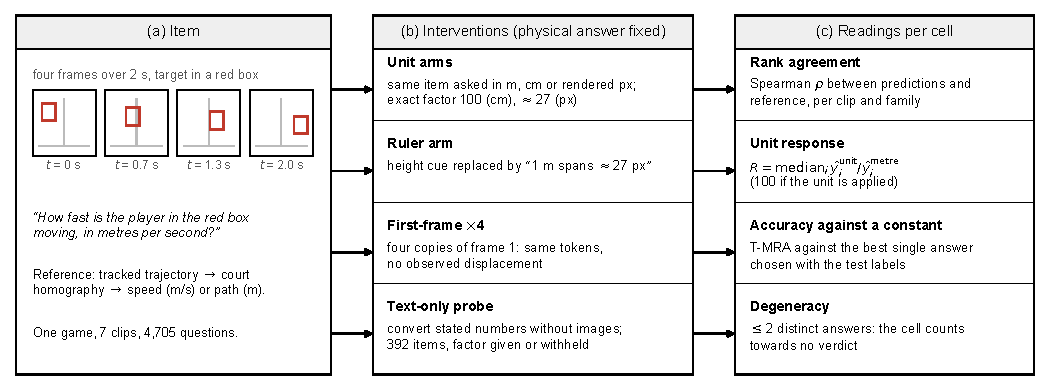
\includegraphics[width=\linewidth]{fig_protocol.pdf}
\caption{The diagnostic protocol: (a)~a CourtDyn item and its
  trajectory-derived reference; (b)~interventions that change the image or
  the requested unit while the physical answer stays fixed; (c)~the readings
  taken from every cell.}
\label{fig:protocol}
\end{figure}
\begin{itemize}
\item \textbf{Unit arms.} The same item is asked in metres, centimetres or
  rendered-image pixels, with the $960\times540$ canvas and the distinction
  between floor-plane and image-plane motion stated in the prompt. Metres and
  centimetres describe the same floor motion, so the exact factor is $100$;
  pixels describe projected motion, whose itemwise reference ratio to metres is
  about $K\approx27$ on the test clips.
\item \textbf{Ruler arm.} The height cue is replaced by ``one meter on the floor
  spans about 27 pixels'', a clip-level scale derived from the homography.
\item \textbf{First-frame$\times4$.} The four frames are replaced by four copies
  of the first: identical token budget, no observed displacement.
\item \textbf{Text-only probes.} Conversions of stated numbers, without images
  (Section~\ref{sec:locate}).
\end{itemize}

\subsection{Metrics}
\label{sec:metric}

For a scalar answer we use the tolerance-based mean relative accuracy
\begin{equation}
\label{eq:tmra}
\mathrm{T\text{-}MRA}(\hat{y}, y) =
\frac{1}{|\Theta|}\sum_{\theta \in \Theta}
\mathbf{1}\!\left[\frac{|\hat{y}-y| - T}{\max(|y|, \epsilon)} < 1-\theta\right],
\end{equation}
with $\Theta = \{0.50, 0.55, \ldots, 0.95\}$, on a $0$--$100$ scale, with $(T,\epsilon)=(0.30,1.0)$ for speed and
$(0.50,2.0)$ for path, scaled with the unit. Each T-MRA is read against a
\emph{test-label constant}: the best single answer for that clip and family,
chosen with knowledge of the test labels. Because it uses the labels, it is a
diagnostic reference rather than a predictor, and exceeding it is a strict
criterion. Rank
agreement is Spearman's \rhosp{} between prediction and reference, per clip and
family, never pooled. Unit response is the paired ratio
\begin{equation}
R = \operatorname{median}_{i}\;\hat y_i^{\mathrm{unit}}/\hat y_i^{\mathrm{metre}}
\label{eq:pairedratio}
\end{equation}
over items where both answers parse and the metre answer is positive. A cell
whose predictions take at most two distinct values is \emph{degenerate}: its
correlation is undefined or uninformative and it never counts towards a
verdict. Intervals are 95\% percentile bootstrap intervals that resample
2-second time windows ($B=2000$), since questions from one window share frames;
resampling players instead gives similar conclusions and is released with the
data.

% ===========================================================================
\section{Experimental setup}
\label{sec:setup}

\paragraph{Backbone and adapters}
All adapters start from public Qwen3.5-4B with NF4 4-bit loading, LoRA
($r=16$, $\alpha=32$) on the language tower and a frozen vision tower, one
epoch at learning rate $10^{-4}$ (\ref{app:training}). CourtDyn-native was
trained on 1,400 v1 speed/path answers from four side clips and one overhead
clip. Two matched adapters were trained on the same ordered 1,120
event-held-out inputs with v1 or v3 labels. All three pools were trained at
seeds 42, 43 and 44.

\paragraph{Event-level split audit}
Two clips of one game can show the same passage of play from different cameras,
so we group clips into events and audit every checkpoint against both test
events by reading the frame identifiers of its frozen training pool
(Table~\ref{tab:splitaudit}). The primary test clip, Q2\_top\_480--510, is
event-disjoint for every checkpoint. The single contaminated cell (the original
native checkpoint on Q1\_top) is excluded from every claim. This is an
event-level holdout within one game; Section~\ref{sec:soccer} provides the
cross-game test.

\begin{table}[t]
\centering\small
\setlength{\tabcolsep}{4pt}
\caption{Event-level split audit. \checkmark: the evaluation event is absent
  from the checkpoint's training pool; $\times$: seen through another camera.
  Generated from the frozen pools.}
\label{tab:splitaudit}
\resizebox{\linewidth}{!}{% Generated by tools/audit_event_splits.py -- do not edit by hand.
\begin{tabular}{lrlcc}
\toprule
 & & & \multicolumn{2}{c}{Evaluation event} \\
\cmidrule(lr){4-5}
Checkpoint & Items & Training clips & Q2\_top & Q1\_top \\
\midrule
CourtDyn-native (original) & 1400 & Q1-side, Q2-side, Q4-side(2), Q4-top & \checkmark & $\times$ \\
Event-holdout v1 (seed 42) & 1120 & Q2-side, Q4-side(2), Q4-top & \checkmark & \checkmark \\
Event-holdout v3 (seed 42) & 1120 & Q2-side, Q4-side(2), Q4-top & \checkmark & \checkmark \\
\bottomrule
\end{tabular}
}
\end{table}

\paragraph{Mixed-unit control}
The v3 pool was rebuilt with exactly half of its 1,120 items asking for
centimetres and carrying the metre answer multiplied by 100, balanced within
every clip and family and chosen by a content hash; items, images, order and
hyperparameters are otherwise identical. Seeds 42, 43 and 44 were trained. The
decision rule, recorded before training (\ref{app:prereg}), counts a cell as
responding if $R\ge10$ and requires three of the four test cells
(Q1/Q2 $\times$ speed/path); it is applied to the explicit prompts and,
separately, to prompts in the training wording.

\paragraph{Second sport and second backbones}
For a cross-game, cross-sport test we took the sequence with the least camera
motion from each of three SoccerNet-GSR matches~\cite{soccernetgsr2024}, whose
annotations give pitch coordinates in metres, and built 140 speed and 140 path
questions per sequence with the same generator and prompts. No adapter saw
soccer. The same training recipe was applied to SmolVLM2-2.2B~\cite{smolvlm2025},
Qwen2.5-VL-3B~\cite{qwen25vl2025}, InternVL3-2B~\cite{internvl3_2025},
Pixtral-12B~\cite{pixtral2024}, Idefics3-8B~\cite{idefics3_2024} and
Gemma3-12B~\cite{gemma3_2025}, with replication rules recorded before training
(Section~\ref{sec:backbones}). InternVL3-2B has its own vision encoder and
multimodal training, but its language model is initialised from Qwen2.5;
Pixtral-12B, Idefics3-8B and Gemma3-12B share no component with the Qwen family
(their language models are from Mistral, Llama~3.1 and Gemma~3). Idefics3-8B
has the architecture and image policy of SmolVLM2-2.2B at a larger scale.

\paragraph{AI-assisted software}
Claude (Anthropic) assisted development of the generator, intervention
builders and analysis scripts; OpenAI Codex assisted auditing and plotting.
All statistics are computed by saved scripts from frozen model outputs; the
evaluated models are objects of study, not tools.

% ===========================================================================
\section{Results}
\label{sec:results}

\subsection{Order is read from motion}
\label{sec:order}

On the event-disjoint clip the CourtDyn-native checkpoint ranks speed and path
with $\rho=0.76$ [$0.70$, $0.82$] and $0.76$ [$0.67$, $0.83$], and its metre
T-MRA ($80.4$/$73.1$) exceeds the median constant of the same clip by $16.6$
[$7.4$, $22.0$] and $19.8$ [$11.1$, $28.2$] points (Tables~\ref{tab:nativecore}
and~\ref{tab:bootstrap}). The ordering does not depend on one seed or one label
convention: across the three matched pools and three seeds, metre $\rho$ spans
$0.66$--$0.80$ in all 18 cells (Table~\ref{tab:seeds}), and the lowest lower
bootstrap limit among them is $0.57$.

The ordering comes from multi-frame content. Replacing the four frames by
copies of the first lowers the native checkpoint's correlations from
$0.76$/$0.76$ to $0.18$/$-0.05$ ($\Delta\rho=+0.59$/$+0.81$), and its distinct
predictions fall from $9$--$13$ to $3$ per cell. Across the seed sweep the
control lowers $\rho$ in all 15 defined cells, by $0.46$--$1.03$. The control
removes most but not all of the ordering: Q2 speed of the native checkpoint
retains a correlation of $0.18$.

\subsection{Magnitude does not follow the unit}
\label{sec:units}

Asked for pixels instead of metres, the native checkpoint keeps its ordering
($\rho=0.70$/$0.73$) but changes its answers by a median factor of $1.11$ and
$0.62$ where the rendered-image convention requires about $27$; its pixel
T-MRA falls to $23.0$/$21.1$, $42.4$ [$34.5$, $51.1$] and $30.7$ [$22.1$, $42.5$]
points below the constant. Supplying the correct scale (``one meter spans
about 27 pixels'') leaves its metre answers unchanged (ratios
$1.00$/$0.67$) and lowers its metre scores to $76.9$/$67.7$.

\begin{table}[t]
\centering\small
\setlength{\tabcolsep}{4pt}
\caption{CourtDyn-native on its event-disjoint clip. T-MRA is model /
  median constant of the clip; $R$ is the paired pixel/metre ratio
  (about $27$ if the unit were applied). Intervals: Table~\ref{tab:bootstrap}.}
\label{tab:nativecore}
\begin{tabular}{lllll}
\toprule
Family & Metre T-MRA & Pixel T-MRA & Pixel $\rho$ & $R$ \\
\midrule
speed & 80.4 / 63.8 & 23.0 / 65.4 & 0.70 & 1.11 \\
path  & 73.1 / 53.3 & 21.1 / 51.8 & 0.73 & 0.62 \\
\bottomrule
\end{tabular}
\end{table}

% Generated by tools/bootstrap_paper2_ci.py -- do not edit by hand.
\begin{table}[t]
\centering\footnotesize
\setlength{\tabcolsep}{4pt}
\caption{95\% cluster-bootstrap intervals for the headline quantities.}
\label{tab:bootstrap}
\begin{tabular}{lll}
\toprule
Quantity (CourtDyn-native, Q2) & speed & path \\
\midrule
metre $\rho$ & 0.76 [0.70, 0.82] & 0.76 [0.67, 0.83] \\
metre margin & 16.6 [7.4, 22.0] & 19.8 [11.1, 28.2] \\
pixel $\rho$ & 0.70 [0.63, 0.76] & 0.73 [0.62, 0.82] \\
pixel margin & -42.4 [-51.1, -34.5] & -30.7 [-42.5, -22.1] \\
pixel/metre $R$ & 1.11 [1.11, 1.13] & 0.62 [0.60, 0.90] \\
\bottomrule
\end{tabular}
\par\vspace{3pt}\begin{flushleft}\footnotesize Time windows resampled, $B=2000$. Margin: T-MRA minus the median constant of the same resample; $R$: paired pixel/metre prediction ratio (about 27 if the unit were applied).\end{flushleft}
\end{table}
% caption trimmed by tools/trim_table_captions.py


The pixel prompt changes the unit and removes the height sentence together,
and pixels measure a different, projected quantity. The cleaner test is
metres against centimetres, which name the same floor motion. With explicit
prompts that state the canvas and the floor/image-plane distinction, the native
checkpoint's centimetre/metre ratios are $1.00$ [IQR $1.00$, $1.80$] for speed
and $1.02$ [$0.90$, $1.60$] for path; without the height sentence both are
$1.00$. Across the 18 seed-sweep cells the ratios are $1.00$--$1.67$, and the
pixel/metre ratios $1.40$--$1.85$ (Table~\ref{tab:seeds}). The answers keep
their order and their metre magnitude whatever unit is requested.

% Generated by tools/analyze_seed_sweep.py -- do not edit by hand.
\begin{table}[t]
\centering\footnotesize
\setlength{\tabcolsep}{3pt}
\caption{Seed variability on the event-disjoint Q2 clip.}
\label{tab:seeds}
\begin{tabular}{lrrrrrrrrr}
\toprule
 & & \multicolumn{4}{c}{speed} & \multicolumn{4}{c}{path} \\
\cmidrule(lr){3-6}\cmidrule(lr){7-10}
Pool & Seed & $\rho$ & T-MRA & cm/m & $\Delta\rho$ & $\rho$ & T-MRA & cm/m & $\Delta\rho$ \\
\midrule
Original & 42 & 0.70 & 77.9 & 1.00 & --- & 0.68 & 70.9 & 1.02 & --- \\
 & 43 & 0.69 & 76.8 & 1.11 & 0.54 & 0.72 & 71.0 & 1.00 & 0.74 \\
 & 44 & 0.76 & 83.4 & 1.11 & 0.75 & 0.79 & 77.1 & 1.00 & 0.52 \\
\addlinespace
v1 labels & 42 & 0.71 & 72.1 & 1.56 & 0.51 & 0.69 & 74.2 & 1.14 & 0.66 \\
 & 43 & 0.66 & 71.1 & 1.67 & 0.46 & 0.72 & 73.1 & 1.00 & 0.65 \\
 & 44 & 0.66 & 73.5 & 1.56 & 0.59 & 0.71 & 60.5 & 1.29 & 0.76 \\
\addlinespace
v3 labels & 42 & 0.76 & 67.6 & 1.57 & --- & 0.77 & 64.1 & 1.00 & 0.74 \\
 & 43 & 0.74 & 68.6 & 1.38 & 0.89 & 0.80 & 59.4 & 1.00 & 1.03 \\
 & 44 & 0.71 & 70.8 & 1.57 & 0.71 & 0.78 & 65.7 & 1.08 & 0.78 \\
\bottomrule
\end{tabular}
\par\vspace{3pt}\begin{flushleft}\footnotesize $\rho$ and T-MRA: metre prompts against v3 references; cm/m: median paired prediction ratio (exact 100); $\Delta\rho$: full minus first-frame$\times4$ (--- undefined or not run). Seeds 43 and 44 retrain seed 42 with identical hyperparameters.\end{flushleft}
\end{table}
% caption trimmed by tools/trim_table_captions.py


\subsection{Where the unit response breaks}
\label{sec:locate}

The most direct alternative explanation is arithmetic: the model reads the
motion but cannot convert. We tested it with 392 text-only items: fourteen
magnitudes from $0.002$ to $400$, three metric conversions in both directions
with the factor stated or withheld, and the metre/pixel conversion at
$K=27.498$, each bare and embedded in the CourtDyn question frame. We score the
246 items on which an unconverted answer would be scored wrong (\supp{2}).

Table~\ref{tab:unit_probe} separates two facts. First, fine-tuning degraded
metric arithmetic: the unadapted backbone answers $80.5\%$ correctly and the
adapters $45.5$--$64.2\%$, each below it on the same items (exact McNemar,
every $p<10^{-7}$); asked for centimetres, every adapter multiplies a stated
metre value by a median of $10$ rather than $100$. Arithmetic therefore
contributes to the centimetre failure. Second, it does not explain the pixel
failure: given $K$, every checkpoint multiplies a stated metre value by a median
of $27.50$, while with the image in view the same adapters return pixel/metre
ratios of $1.45$--$1.83$. The conversion they apply to a stated number is not
applied to the number they read from the image. The unadapted backbone cannot
test the image side: on these clips its answers take one to three distinct
values per arm, with every defined $\rho<0.13$; fine-tuning is what makes the
model read motion at all.

% Generated by tools/analyze_unit_probe.py -- do not edit by hand.
\begin{table}[t]
\centering\small
\setlength{\tabcolsep}{3pt}
\caption{Text-only unit conversion against the same checkpoints' visual unit responses, Q2.}
\label{tab:unit_probe}
\begin{tabular}{lrrrrrr}
\toprule
 & & & \multicolumn{2}{c}{cm/m} & \multicolumn{2}{c}{px/m} \\
\cmidrule(lr){4-5}\cmidrule(lr){6-7}
Checkpoint & Text acc.\ (\%) & $p$ vs base & text & image & text & image \\
\midrule
Base (no adapter) & 80.5 [75.1, 85.0] & --- & 100.0 & degen. & 27.50 & degen. \\
CourtDyn-native & 45.5 [39.4, 51.8] & $3.2\times10^{-22}$ & 10.0 & 1.00/1.02 & 27.50 & 1.60/1.80 \\
Event-holdout v1 & 64.2 [58.1, 70.0] & $1.0\times10^{-8}$ & 10.0 & 1.56/1.14 & 27.50 & 1.67/1.55 \\
Event-holdout v3 & 58.1 [51.9, 64.1] & $2.0\times10^{-10}$ & 10.0 & 1.57/1.00 & 27.50 & 1.83/1.45 \\
\bottomrule
\end{tabular}
\par\vspace{3pt}\begin{flushleft}\footnotesize Accuracy on the 246 diagnostic items (Wilson 95\% intervals); $p$: exact McNemar against the unadapted backbone. Ratios: median requested-unit answer over the metre quantity (text: the stated value; image arms: the metre-arm answer); required cm/m $=100$, px/m $=27.50$. Base image arms are degenerate (1--3 distinct answers).\end{flushleft}
\end{table}
% caption trimmed by tools/trim_table_captions.py


This dissociation suggests a training-free remedy: ask for metres from the
image, then pass that answer back verbatim in a text-only turn with the
conversion factor. Three predictions were recorded from the text probe alone
before the run (\ref{app:prereg}): pixel conversion reaches the exact-conversion
ceiling for every checkpoint (H1); centimetre conversion falls at least 20 T-MRA
points short of it for the adapters (H2); the backbone converts centimetres
correctly (H3). H1 holds in all eight checkpoint--family cells: pixel-target
T-MRA rises from $21.6$--$23.4$ under the direct prompt to $63.9$--$77.8$,
within $0.2$ points of the ceiling (Table~\ref{tab:two_stage}). H3 holds. H2
holds in five of six cells; for v3 path the shortfall is $17.7$ points, a partial
recovery. The magnitude the adapters read from the image is therefore good
enough to support a correct pixel answer; what is missing is the step that
applies the unit to it.

% Generated by tools/analyze_two_stage_units.py -- do not edit by hand.
% v2 copy: only change is \resizebox to the text width (Neurocomputing layout, 2026-09-28).
\begin{table}[t]
\centering\small
\setlength{\tabcolsep}{3pt}
\caption{Two-stage unit answering on Q2: direct, two-stage and ceiling T-MRA.}
\label{tab:two_stage}
\resizebox{\linewidth}{!}{%
\begin{tabular}{llrrrrrrr}
\toprule
 & & \multicolumn{3}{c}{speed T-MRA} & \multicolumn{3}{c}{path T-MRA} & \\
\cmidrule(lr){3-5}\cmidrule(lr){6-8}
Checkpoint & Unit & direct & two-stage & ceiling & direct & two-stage & ceiling & ratio \\
\midrule
Base (no adapter) & px & 18.7 & 23.4 & 23.4 & 18.4 & 24.8 & 24.8 & 27.5/27.5 \\
 & cm & 17.5 & 23.4 & 23.4 & 18.6 & 24.5 & 24.5 & 100.0/100.0 \\
\addlinespace
CourtDyn-native & px & 23.1 & 77.8 & 77.9 & 21.6 & 70.9 & 70.9 & 27.4/27.5 \\
 & cm & 21.3 & 25.1 & 77.9 & 20.2 & 22.9 & 70.9 & 10.0/10.0 \\
\addlinespace
Event-holdout v1 & px & 23.4 & 71.9 & 72.0 & 23.4 & 73.8 & 73.7 & 27.4/27.5 \\
 & cm & 21.4 & 24.9 & 72.1 & 20.4 & 24.8 & 74.2 & 10.0/10.0 \\
\addlinespace
Event-holdout v3 & px & 23.1 & 67.8 & 67.9 & 21.7 & 63.9 & 63.9 & 27.5/27.5 \\
 & cm & 21.6 & 23.7 & 67.6 & 20.2 & 46.4 & 64.1 & 10.0/55.0 \\
\bottomrule
\end{tabular}}
\par\vspace{3pt}\begin{flushleft}\footnotesize Direct: target unit asked from the image. Two-stage: the model's own metre answer passed back in a text-only turn with the conversion factor. Ceiling: that metre answer converted exactly. T-MRA against the target arm's references; ratio: median two-stage answer over metre answer (required px $27.50$, cm $100$). Base metre answers are degenerate. Predictions recorded before the second stage ran (\supp{2}).\end{flushleft}
\end{table}
% caption trimmed by tools/trim_table_captions.py


\subsection{The cause: single-unit supervision}
\label{sec:m1}

Every adapter above was trained on metre answers only. ``Ask for centimetres,
get the metre number'' is then predicted by answer-distribution fitting alone,
without any account of how the image is read. The mixed-unit control tests this
directly (Table~\ref{tab:m1}).

% Generated by tools/make_paper2_v2_tables.py -- do not edit by hand.
\begin{table}[t]
\centering\footnotesize
\setlength{\tabcolsep}{3pt}
\caption{Mixed-unit supervision at three seeds, explicit prompts.}
\label{tab:m1}
\resizebox{\linewidth}{!}{%
\begin{tabular}{llrrrrrrr}
\toprule
 & & \multicolumn{3}{c}{$R$} & \multicolumn{3}{c}{$\rho_{\mathrm{cm}}$} & Median / prior \\
\cmidrule(lr){3-5}\cmidrule(lr){6-8}
Family & Event & s42 & s43 & s44 & s42 & s43 & s44 & (s42--44) \\
\midrule
path & Q1 & 100 & 76 & 100 & 0.69 & 0.64 & 0.64 & 160/130/140 / 215 \\
path & Q2 & 100 & 76 & 100 & 0.70 & 0.64 & 0.70 & 120/110/140 / 215 \\
\addlinespace
speed & Q1 & 183$^{*}$ & 183$^{*}$ & 183$^{*}$ & 0.37 & --- & --- & 110/110/110 / 110 \\
speed & Q2 & 250$^{*}$ & 183$^{*}$ & 183 & 0.61 & 0.15 & 0.27 & 100/110/110 / 110 \\
\bottomrule
\end{tabular}}
\par\vspace{3pt}\begin{flushleft}\footnotesize $R$: median paired cm/m ratio (exact $=100$); $^{*}$: degenerate centimetre arm, excluded from verdicts; $\rho_{\mathrm{cm}}$: Spearman correlation of the centimetre answers (--- undefined); Median: centimetre answers against the training-pool median of centimetre targets.\end{flushleft}
\end{table}
% caption trimmed by tools/trim_table_captions.py


For path length the unit response is restored. With explicit prompts the
centimetre/metre ratio is $100$ in four of six seed--event cells and $76$ in the
other two, against $1.00$ for the metre-only adapter; the centimetre answers
keep ranking the motion ($\rho_{\mathrm{cm}}=0.64$--$0.70$, close to the metre
arm), and their medians follow the metre answers rather than the centimetre
training median. The same holds in the training wording (ratios $69$--$100$).
Mixed-unit training also restores text arithmetic: on the 246 diagnostic items
the adapter answers $83.7\%$ [$78.6$, $87.8$], indistinguishable from the
unadapted backbone ($80.5\%$, $p=0.15$) and far above the metre-only v3 adapter
($58.1\%$, $p=9.7\times10^{-14}$). The arithmetic damage of
Section~\ref{sec:locate} is therefore also a consequence of metre-only
supervision on this backbone; Section~\ref{sec:backbones} shows that it does
not hold on every backbone.

For speed the outcome differs. Under the rule as first recorded, seed 42
satisfied the criterion in both wordings because its speed ratios were large
($183$ and $250$), but its centimetre speed answers took only two distinct
values. The degeneracy rule used throughout the study was therefore added to
the M1 rule, post hoc for seed 42 and before seeds 43 and 44 were trained
(\ref{app:prereg}). Under it, path supports the supervision account in all
three seeds and speed in none: 11 of 12 speed cells across seeds and wordings
are degenerate. Section~\ref{sec:prior} identifies what the speed ratios
measure.

Mixed-unit supervision has a cost in metre accuracy, as expected when half of
the metre targets are replaced. Against the metre-only adapter of the same
seed, it lowers Q2 metre speed T-MRA in all three seeds, by $7.2$--$15.1$
points, and lowers metre $\rho$ in all six Q2 cells, by $0.03$--$0.24$; for
path T-MRA the change is $-4.8$ and $-8.9$ in two seeds and $+5.0$ in the
third. The pixel unit, never seen in training, is not repaired: the mixed-unit
adapter answers pixel path questions with ratios near $100$ ($84.6$ and
$100.0$ at seed 42), consistent with a learned rule that any non-metre unit
scales the metre answer by 100, and pixel speed with $2.3$--$2.8$.

\subsection{Speed: the answer distribution of a unit}
\label{sec:prior}

The mixed-unit speed ratios are not conversions. In five of the six
explicit-prompt speed cells the median centimetre answer is $110$ (in the
sixth, $100$), which is the median of the centimetre speed targets in the
training pool (whose most frequent values are $80$--$120$), while the same
adapter's metre answers have medians of $0.4$--$0.6$\,m/s. The ratio of
$183$ is $110/0.6$. The centimetre answers barely rank the motion
($\rho_{\mathrm{cm}}$ at most $0.61$ and undefined in two cells), while the
metre answers of the same adapter keep $\rho=0.48$--$0.67$ on Q2. For path,
by contrast, the centimetre medians ($110$--$160$) track the metre answers and
stay far from the centimetre training median of $215$.

\begin{figure}[t]
\centering
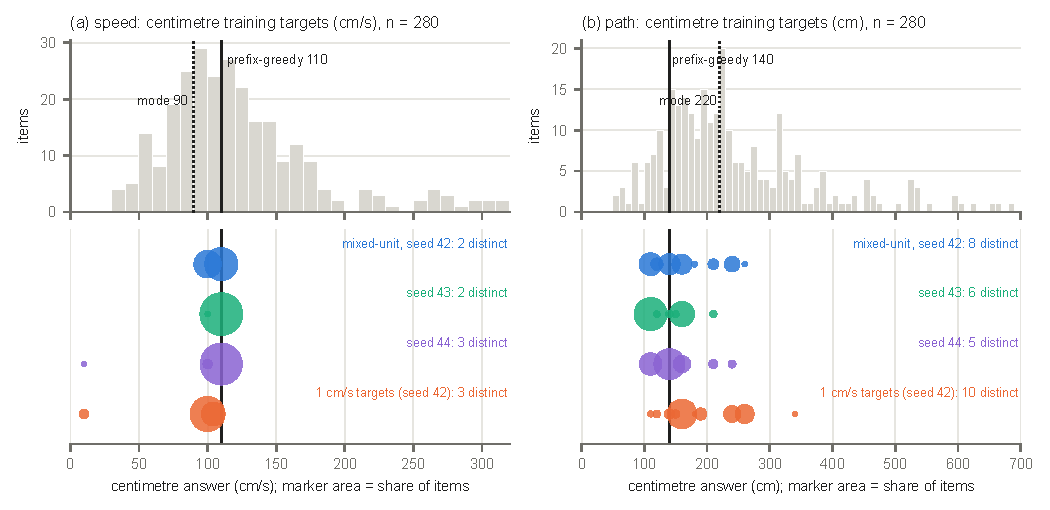
\includegraphics[width=\linewidth]{fig_speed_collapse.pdf}
\caption{Centimetre answers of the mixed-unit adapters for (a)~speed and
  (b)~path. Top: centimetre training targets with their prefix-greedy value
  (solid) and mode (dotted). Bottom: answers at seeds 42--44 and after the
  1\,cm/s retraining; marker area is the share of items. Speed collapses onto
  the prefix-greedy value ($110$); path spreads with the motion.}
\label{fig:collapse}
\end{figure}

The two families thus bound what mixed supervision teaches
(Fig.~\ref{fig:collapse}). Where it succeeds,
the adapter converts its own reading; where it fails, it has learned the
distribution of answers that come with the word ``centimetres'' and returns the
centre of that distribution. The same account explains the metre-only adapters'
behaviour in Section~\ref{sec:units}, whose answers stay in the metre range
whatever unit is asked: in both cases the numeric output is anchored to a
per-unit answer distribution learned in fine-tuning, and only where the
supervision ties the two units to the same items does a conversion emerge.

Why path and speed differ is not the resolution of the targets. Both families
come from the same windows with the same relative spread, but every
centimetre target was the one-decimal metre answer times 100, a coarser grid
relative to speed than to path. A preregistered follow-up retrained the
seed-42 mixed-unit adapter with the centimetre speed targets at 1\,cm/s, all
else identical (\ref{app:prereg}). The speed collapse remained: the
centimetre answers have a median of $100$, take two or three distinct values,
and barely track the reference ($\rho_{\mathrm{cm}}=0.10$ and $0.18$), while path
still converts ($R=119$--$127$, $\rho_{\mathrm{cm}}=0.60$--$0.64$). The
difference between the families remains unexplained.

The collapsed value itself can be read off the training targets (a post hoc
analysis). The backbone's
tokenizer emits numbers one digit at a time, so greedy decoding of an output
that does not depend on the image returns not the most frequent centimetre
target but its digit-by-digit majority: the majority first digit, then the
majority second digit among the targets that share that prefix, and so on.
For the centimetre speed targets this prefix-greedy value is $110$ (half of
the targets begin with a 1, and among those $110$ leads), whereas their mode
is $90$; for the 1\,cm/s targets of the retraining it is $100$, whereas their
mode is $79$. The adapters answer exactly these values: $110$ in $44$--$100\%$
of the items of each speed cell across the three seeds ($100$ otherwise), and
$100$ or $104$ after the 1\,cm/s retraining ($65$--$67\%$). Conditioning the
same prediction on the adapter's own metre reading of each item does not
improve it (at most $14\%$ agreement), so the centimetre speed channel does
not read the image at all. The path targets spread over more first digits
($37\%$ share the majority first digit, against $50\%$ for speed); their
prefix-greedy value, $140$, is one of several answers the adapters give,
alongside converted values. Whether the strength of this prefix prior
determines which families mixed supervision can repair is a hypothesis for
future work, formed after these results.

\subsection{Reading, then converting}
\label{sec:rtc}

The text routing of Section~\ref{sec:locate} needs a second turn. A
preregistered follow-up asked whether the conversion can be folded into one
answer. The adapter is trained on the mixed-unit pool with every target
rewritten as ``\emph{reading in metres} m $\rightarrow$ \emph{value}
\emph{unit}'' (read-then-convert, RTC), and the decisive test is conversion to
units that never occur in training: km/h and ft/s for speed, ft and mm for
path. A cell converts if the paired ratio lies within $[f/1.5,\,1.5f]$ of the
exact factor $f$, the arm is non-degenerate and $\rho\ge0.30$; the hypothesis
holds with six of eight cells (\ref{app:prereg}). Two controls were recorded
with it: the metre-only and mixed-unit adapters asked in the RTC output format
without any RTC training (the format control), and the RTC adapter's metre
ranking against the metre-only adapter's.

On Qwen3.5-4B the output format accounts for most of the effect. Without
training, the metre-only adapter converts six of the eight unseen-unit cells at every seed
and the mixed-unit adapter six, five and six. The RTC-trained adapter converts
eight of eight at seed 42 but five and four at seeds 43 and 44, so the gain of
training over the format is seed-dependent. It converts centimetre speed at
all three seeds, the family that mixed supervision could not repair, and its
metre ranking is not inferior to the metre-only adapter's at one seed of
three.

On the other backbones the format trades reading for conversion. The
RTC-trained InternVL3-2B, Pixtral-12B and Gemma3-12B adapters return ratios at
the exact factor in most cells, but their metre answers lose their ordering or
collapse, so they convert in zero, one and three cells of eight; Pixtral's
metre path readings take two distinct values. The format control converts nothing on
the three metre-only adapters and five cells on Pixtral's mixed-unit adapter.
Per-cell ratios and rank correlations are in \supp{5}. We therefore report RTC
as a prompting effect of this backbone, not as a training method.

\subsection{A linear probe of the hidden states}
\label{sec:probe}

A preregistered probe asked whether the reference quantity can be read
linearly from the hidden states of the unadapted backbone and of the
CourtDyn-native, metre-only v3 and mixed-unit adapters, and whether that readout
depends on the motion in the frames. It can be read in every model (10 of 10
cross-validation fold seeds in both families, against a permutation null). Its
motion dependence, however, appears only after metre-only fine-tuning: under
first-frame repetition the readout of the v3 adapter loses its correlation in
10 of 10 fold seeds in both families (CourtDyn-native: 10 and 9), while the
unadapted backbone's and the mixed-unit adapter's keep it (0 of 10). Whether
the readout is closer to the image-plane or the floor-plane quantity is not
stable across fold seeds and is not interpreted; the preregistered single-seed
analysis and the post hoc ten-seed check are both in \supp{5}. The probe
agrees with the behavioural picture: metre-only
fine-tuning makes the internally readable quantity motion-dependent without
making the numeric output unit-dependent.

\subsection{A second sport, zero-shot}
\label{sec:soccer}

Table~\ref{tab:soccer} evaluates the basketball adapters zero-shot on three
soccer matches, a cross-game and cross-sport test reported descriptively (no
decision rule was recorded for it). The metre-only adapter reproduces every
part of the dissociation. It ranks motion in all six
cells, with $\rho=0.33$--$0.78$ and every bootstrap interval above zero; the
highest correlations are on the sequence with an almost static camera
(SNGS-056, $0.74$/$0.78$), the lowest on SNGS-034 ($0.33$/$0.40$), one of the
two whose camera moves (median 21 and 24 pixels per two seconds). The
first-frame control lowers $\rho$ in all six cells ($\Delta\rho$
$0.35$--$0.63$). Its centimetre/metre ratios are $1.0$--$1.2$ and its
pixel/metre ratios $1.00$--$1.83$ against $K=20.8$--$30.4$. Its metre T-MRA is
within $-3.2$ to $+3.7$ points of the best test-label constant, so it does not
measure the soccer magnitudes better than a constant does, although it orders
them.

% Generated by tools/make_paper2_v2_tables.py -- do not edit by hand.
\begin{table}[t]
\centering\footnotesize
\setlength{\tabcolsep}{2.5pt}
\caption{Second sport, zero-shot: three SoccerNet-GSR matches.}
\label{tab:soccer}
\resizebox{\linewidth}{!}{%
\begin{tabular}{lllrrrrr}
\toprule
Adapter & Match ($K$) & Family & $\rho$ & $\Delta\rho$ & Margin & cm/m & px/m \\
\midrule
metre-only & SNGS-034 (20.8) & speed & 0.33 [0.18, 0.44] & 0.39 & 1.0 & 1.0 & 1.22 \\
metre-only & SNGS-034 (20.8) & path & 0.40 [0.24, 0.52] & 0.44 & -0.4 & 1.0 & 1.00 \\
metre-only & SNGS-056 (30.4) & speed & 0.74 [0.61, 0.84] & 0.45 & -2.3 & 1.0 & 1.57 \\
metre-only & SNGS-056 (30.4) & path & 0.78 [0.67, 0.85] & 0.54 & -3.2 & 1.1 & 1.55 \\
metre-only & SNGS-096 (26.1) & speed & 0.59 [0.43, 0.72] & 0.35 & -2.4 & 1.2 & 1.83 \\
metre-only & SNGS-096 (26.1) & path & 0.56 [0.41, 0.68] & 0.63 & 3.7 & 1.1 & 1.44 \\
\addlinespace
mixed-unit & SNGS-034 (20.8) & speed & 0.28 & 0.17 & -0.1 & 137.5$^{*}$ & 1.38 \\
mixed-unit & SNGS-034 (20.8) & path & 0.28 & 0.09 & 0.9 & 87.5 & 68.75 \\
mixed-unit & SNGS-056 (30.4) & speed & 0.71 & 0.43 & -7.9 & 166.7$^{*}$ & 1.83 \\
mixed-unit & SNGS-056 (30.4) & path & 0.71 & 0.53 & -12.0 & 100.0 & 90.91 \\
mixed-unit & SNGS-096 (26.1) & speed & 0.58 & 0.30 & -2.4 & 250.0 & 2.75 \\
mixed-unit & SNGS-096 (26.1) & path & 0.50 & 0.32 & 3.4 & 100.0 & 76.92 \\
\bottomrule
\end{tabular}}
\par\vspace{3pt}\begin{flushleft}\footnotesize Basketball-trained Qwen3.5-4B adapters; no decision rule was recorded. $\rho$ with 95\% window-clustered bootstrap interval; $\Delta\rho$: full minus first-frame$\times4$; margin: metre T-MRA minus the best test-label constant; $R$: paired ratios.\end{flushleft}
\end{table}
% caption trimmed by tools/trim_table_captions.py


The mixed-unit adapter transfers the same split as in basketball: path
centimetre ratios of $87.5$--$100$, speed centimetre answers degenerate in two
matches and at $250$ in the third, and pixel path ratios of $69$--$91$ rather
than $K$. Its metre ranking is lower than the metre-only adapter's in all six
cells.

\subsection{Other backbones}
\label{sec:backbones}

We applied the same recipe to SmolVLM2-2.2B and Qwen2.5-VL-3B, with rules R1--R4
recorded before training (Table~\ref{tab:backbones}): R1, the metre-only adapter
orders motion ($\rho\ge0.30$) without converting units ($R\le3$); R2, the
mixed-unit adapter converts ($R\ge10$); R3, text arithmetic is damaged by
metre-only and not by mixed-unit training; R4, first-frame repetition lowers
$\rho$. Each is decided on four cells, and a rule with fewer than three
non-degenerate cells is untestable (the preregistration's LIMITED label).

% Generated by tools/make_paper2_v2_tables.py -- do not edit by hand.
\begin{table}[t]
\centering\footnotesize
\setlength{\tabcolsep}{3pt}
\caption{Other backbones under rules R1--R4 recorded before training.}
\label{tab:backbones}
\resizebox{\linewidth}{!}{%
\begin{tabular}{llllllll}
\toprule
Backbone & Round & Epoch & R1 & R2-E & R2-T & R3 & R4 \\
\midrule
SmolVLM2-2.2B & 1 & 1 & untestable (2) & untestable (2) & replicates (4) & fails & untestable (2) \\
 & 2 & 4$^\dagger$ & intermediate (4) & untestable (2) & intermediate (3) & fails & intermediate (4) \\
Qwen2.5-VL-3B & 1 & 1 & untestable (0) & untestable (0) & untestable (2) & intermediate & untestable (0) \\
 & 2 & 4 & intermediate (4) & intermediate (3) & intermediate (4) & replicates & untestable (2) \\
InternVL3-2B & 2 & 2 & intermediate (3) & untestable (2) & replicates (3) & fails & replicates (4) \\
Pixtral-12B & 2 & 2 & replicates (4) & intermediate (3) & untestable (1) & replicates & untestable (2) \\
Idefics3-8B & 2 & 2 & untestable (1) & intermediate (4) & intermediate (3) & intermediate & untestable (1) \\
Gemma3-12B & 2 & 2 & fails (4) & untestable (2) & intermediate (4) & fails & replicates (4) \\
\bottomrule
\end{tabular}}
\par\vspace{3pt}\begin{flushleft}\footnotesize In parentheses: non-degenerate cells of four; untestable = fewer than three. $^\dagger$Degenerate at the four-epoch cap (descriptive only). Rounds and protocols: Section~\ref{sec:backbones}.\end{flushleft}
\end{table}
% caption trimmed by tools/trim_table_captions.py


After one epoch (round 1), neither backbone reads motion: most metre cells take
one or two distinct answers, as do the unadapted backbones, so R1, R2 and R4
are untestable. SmolVLM2's in-template R2 satisfies the ratio criterion, but its
centimetre answers do not track the reference ($\rho_{\mathrm{cm}}$ from
$-0.32$ to $0.03$): metre answers near a constant $1.8$ and centimetre answers
near $150$--$180$ give a ratio near 100 without any reading, which is the
failure Section~\ref{sec:prior} describes. The round-2 rule adds a tracking
condition to R2 for this reason. On text arithmetic, Qwen2.5-VL-3B shows the
Qwen3.5 direction: metre-only training lowers diagnostic accuracy from
$56.1\%$ to $30.5\%$ ($p=3.5\times10^{-14}$), mixed-unit training to $48.0\%$
($p=0.0055$), so the damage is smaller but not absent (R3 intermediate).
SmolVLM2's backbone answers only $11.8\%$ and fine-tuning raises it, so R3 is
not applicable there.

One epoch was tuned for the 4B backbone, so round 1 cannot distinguish a
smaller model that does not read motion from one that was under-trained. In
round 2 the training length was chosen per backbone on a development clip that
is neither in training nor a test cell, using only answer diversity: the
smallest epoch, up to four, at which the metre-only adapter gives at least five
distinct answers in each family (\ref{app:prereg}).
SmolVLM2 never met this criterion at any of three seeds (at epoch four its
metre-only adapter gives one to four distinct answers per family), so it is
degenerate at the four-epoch cap and its round-2 cells are descriptive only: at
seed 42 metre $\rho$ is $0.06$--$0.19$, and first-frame repetition lowers $\rho$
in one of four cells. Under this recipe it marks a scale boundary rather than a
replication.

Under this criterion Qwen2.5-VL-3B (epoch four), InternVL3-2B, Pixtral-12B,
Idefics3-8B and Gemma3-12B (epoch two) all read motion; SmolVLM2-2.2B does
not. Their per-cell numbers at seed 42 are in \supp{5}; Table~\ref{tab:backbones}
gives the verdicts, and Table~\ref{tab:seeds} repeats the rules at seeds 43
and 44 with the schedule selected at seed 42 (\ref{app:prereg}) for every
trained backbone, together with the label across seeds fixed before seeds 43
and 44 were run.

% Generated by tools/make_paper2_extra_tables.py -- do not edit by hand.
\begin{table}[t]
\centering\footnotesize
\setlength{\tabcolsep}{2.5pt}
\caption{Other backbones at seeds 42 / 43 / 44 under the preregistered rules, with the label across seeds.}
\label{tab:seeds}
\resizebox{\linewidth}{!}{%
\begin{tabular}{lcccccc}
\toprule
Backbone & seeds & R1 & R2-E & R2-T & R3 & R4 \\
\midrule
Qwen2.5-VL-3B & 3 & int. / rep. / int. (n.e.) & int. / unt. / int. (n.e.) & int. / int. / int. (n.e.) & rep. / rep. / rep. (3/3) & unt. / rep. / rep. (2/3) \\
InternVL3-2B & 3 & int. / rep. / rep. (2/3) & unt. / unt. / rep. (n.e.) & rep. / unt. / rep. (2/3) & fails / fails / fails (fails) & rep. / rep. / rep. (3/3) \\
Pixtral-12B & 3 & rep. / rep. / rep. (3/3) & int. / rep. / rep. (2/3) & unt. / int. / unt. (n.e.) & rep. / fails / rep. (s.-d.) & unt. / rep. / rep. (2/3) \\
Idefics3-8B & 3 & unt. / rep. / int. (n.e.) & int. / int. / unt. (n.e.) & int. / int. / int. (n.e.) & int. / rep. / rep. (2/3) & unt. / rep. / int. (n.e.) \\
Gemma3-12B & 3 & fails / int. / rep. (s.-d.) & unt. / unt. / unt. (n.e.) & int. / int. / int. (n.e.) & fails / fails / fails (fails) & rep. / rep. / rep. (3/3) \\
SmolVLM2-2.2B$^\dagger$ & 3 & int. / int. / unt. (n.e.) & unt. / unt. / unt. (n.e.) & int. / unt. / unt. (n.e.) & fails / fails / fails (fails) & int. / int. / int. (n.e.) \\
\bottomrule
\end{tabular}}
\par\vspace{3pt}\begin{flushleft}\footnotesize Cells: seed 42 / 43 / 44; rep.\ = replicates, int.\ = intermediate, unt.\ = untestable. In parentheses the label across seeds: 3/3; 2/3 (holds at two, fails at none); fails; s.-d.\ (seed-dependent); n.e.\ (not established). Seeds 43 and 44 use the schedule selected at seed 42. $^\dagger$Descriptive only.\end{flushleft}
\end{table}
% caption trimmed by tools/trim_table_captions.py


Zero-shot, before any fine-tuning, nine public backbones answer the same
explicit unit cells (\supp{5}). Only InternVL3-8B and Qwen2.5-VL-7B move with
the unit ($R_{\mathrm{cm}}=19$--$58$ and $25$--$104$ in their non-degenerate
cells) while barely ranking the motion (metre $\rho\le0.50$); the others
return near-constant answers. One cell of that sweep is invalid (the bf16
Qwen3.5-4B run left the model's thinking mode on and produced no answer) and
is marked as such.

Taken together (Fig.~\ref{fig:unitsrank}), the rules replicate on some
backbones and not on others, and we state each by its label across seeds
(Table~\ref{tab:seeds}). The unit non-response of the metre-only adapter (R1)
\seedlabel{pixtral_12b}{R1} on Pixtral-12B, a family unrelated to Qwen
(\seeddetail{pixtral_12b}{R1}). It
\seedlabel{internvl3_2b}{R1} on InternVL3-2B (\seeddetail{internvl3_2b}{R1})
and \seedlabel{qwen25vl3b}{R1} on Qwen2.5-VL-3B
(\seeddetail{qwen25vl3b}{R1}); at seed 42 no metre-only path cell converts on
either ($R\le1.20$). On Gemma3-12B it \seedlabel{gemma3_12b}{R1}
(\seeddetail{gemma3_12b}{R1}): three of four cells convert at seed 42, the two
path cells at seed 43 ($R=70.9$ and $10.5$), none at seed 44. It cannot be
tested on SmolVLM2-2.2B, and on Idefics3-8B it \seedlabel{idefics3_8b}{R1}
(\seeddetail{idefics3_8b}{R1}). The first-frame dependence of the ordering
(R4), established on Qwen3.5-4B, holds at all three seeds on InternVL3-2B and
Gemma3-12B; on Pixtral-12B it \seedlabel{pixtral_12b}{R4}
(\seeddetail{pixtral_12b}{R4}; at seed 42 Pixtral-12B orders motion in every
cell but its path answers become constant under the first-frame control), on
Qwen2.5-VL-3B it \seedlabel{qwen25vl3b}{R4} (\seeddetail{qwen25vl3b}{R4}), and
on Idefics3-8B it \seedlabel{idefics3_8b}{R4} (\seeddetail{idefics3_8b}{R4}).
At seed 42, arithmetic damage after metre-only training appears on four of
seven backbones (Qwen3.5-4B, Qwen2.5-VL-3B, Pixtral-12B, Idefics3-8B), is
absent on Gemma3-12B and reverses on InternVL3-2B and on SmolVLM2-2.2B, whose
unadapted backbone answers only $11.8\%$. Across seeds, R3 fails on InternVL3-2B
and Gemma3-12B, \seedlabel{pixtral_12b}{R3} on Pixtral-12B
(\seeddetail{pixtral_12b}{R3}), \seedlabel{qwen25vl3b}{R3} on
Qwen2.5-VL-3B (\seeddetail{qwen25vl3b}{R3}) and \seedlabel{idefics3_8b}{R3} on
Idefics3-8B (\seeddetail{idefics3_8b}{R3}). Post hoc, the one backbone whose
metre-only adapter converts at some seed, Gemma3-12B, keeps its arithmetic at
every seed, but InternVL3-2B keeps its arithmetic without converting, so the
two properties are not read as one mechanism. The pattern of the primary
backbone therefore holds across families where its rules can be judged, with
the exceptions stated above; the backbones do not support a statement about
vision--language models in general.

\begin{figure}[t]
\centering
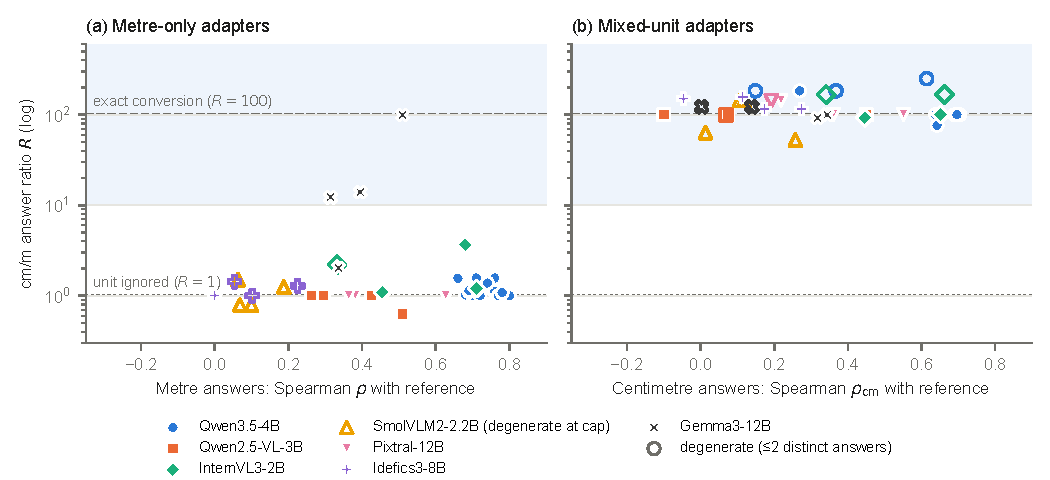
\includegraphics[width=\linewidth]{fig_units_vs_rank.pdf}
\caption{Unit response $R$ (median paired cm/m answer ratio; exact $=100$,
  band $R\ge10$) against rank agreement for every adapter cell at seed 42.
  (a)~Metre-only adapters; (b)~mixed-unit adapters, explicit prompts.
  Metre-only adapters that order the motion sit at $R\approx1$ on every
  backbone except Gemma3-12B; mixed-unit adapters reach $R\approx100$ for path
  and collapse for speed.}
\label{fig:unitsrank}
\end{figure}

% ===========================================================================
\section{Discussion}
\label{sec:discussion}

\paragraph{What a fine-tuned number is}
The adapters read something real from the frames: the ordering survives three
seeds, two label conventions, a change of sport and a second vision stack, and
it disappears when
the motion is removed. The magnitude attached to that ordering behaves
differently. It lives on the scale of the unit the adapter was trained in; it
does not move when another unit is requested; and when a second unit is
supervised, it moves only where that supervision tied the two units to the same
readings. In summary, fine-tuning taught a per-unit answer distribution and
an ordering, and a conversion only where the data forced one.
The static-image companion study~\cite{ji2026calibration} found adaptation
repairing the calibration of an answer distribution rather than localisation;
the present results show the same kind of repair along the unit axis.

\paragraph{Implications for evaluation}
Three practices follow, none requiring new annotation. Report every metric cell
against a test-label constant and a rank correlation, because the adapters here
reach tolerance scores within a few points of a constant on soccer while
ranking the motion well. Test the response to the requested unit, which a
single-unit benchmark never exercises. Report degeneracy explicitly: two of our
own decision rules, as first written, passed on ratios produced by constant
answers, and in both cases only an inspection of the answer distribution
revealed it.

\paragraph{Implications for training}
Single-unit supervision is a property of most domain fine-tuning sets. Where
units matter, mixing units on the same items restores conversion for some
quantities and not others, and costs metre accuracy on speed; routing the
model's own reading through a text-only conversion restores the pixel unit at no
training cost, because the arithmetic on stated numbers is intact where the
supervision did not damage it. Asking for the reading and the converted value
in one answer does the same for units never seen in training, but only on the
backbone it was developed on; elsewhere the format costs the reading.

% ===========================================================================
\section{Limitations}
\label{sec:limits}

\begin{enumerate}
\item \textbf{Backbone.} The full set of results comes from one 4B backbone.
  The other backbones were run at three seeds each (Table~\ref{tab:seeds});
  on Gemma3-12B the unit non-response
  \seedlabel{gemma3_12b}{R1}, on Idefics3-8B it \seedlabel{idefics3_8b}{R1}
  (\seeddetail{idefics3_8b}{R1}), and SmolVLM2-2.2B is degenerate at the
  four-epoch cap at all three seeds. The arithmetic
  damage is backbone-dependent, and the read-then-convert format is a property
  of Qwen3.5-4B. We claim a behaviour of these adapters, not of VLMs in
  general.
\item \textbf{Data.} Training and the basketball tests use one game; the soccer
  test adds three matches but is descriptive, uses three short sequences, and
  two of them have moving cameras. The splits are event-level within the game
  and audited per checkpoint.
\item \textbf{What is identified.} Rank agreement without unit response is a
  behavioural dissociation; the probe of Section~\ref{sec:probe} shows a
  motion-dependent readout, not a measurement mechanism. Why mixed supervision
  converts path but not speed is not identified; the prefix-prior account of
  Section~\ref{sec:prior} is post hoc.
\item \textbf{References.} The court homography is inflated by about $1\%$,
  which leaves ranks unchanged; the timing family has no usable homography
  reference and is excluded; bootstrap intervals resample time windows and do
  not account for the single game.
\item \textbf{Cost.} Mixed-unit training lowers metre accuracy on speed; we did
  not search for a mixing ratio that avoids it.
\end{enumerate}

% ===========================================================================
\section{Conclusion}

Fine-tuned VLMs in this study read the order of motion from video and attach to
it a magnitude that belongs to the unit they were trained in. Mixed-unit
supervision shows that the unit non-response is caused by single-unit training,
repairs it where the supervision ties the units to the same items, and exposes
the other outcome, an answer distribution per unit, where it does not. A
tolerance score, even one well above chance, does not distinguish these; a
constant baseline, a rank correlation, a unit intervention and a first-frame
control do, and none needs new annotation. The protocol applies unchanged to
any domain whose answers derive from tracked trajectories, which is the
subject of ongoing work.

\section*{CRediT authorship contribution statement}
\textbf{Jun Ji:} Data curation, Methodology, Formal analysis, Resources,
Writing -- original draft. \textbf{Bowen Tan:} Software, Formal analysis,
Writing -- review \& editing. \textbf{Yizhou Zhao:} Software, Formal analysis,
Writing -- review \& editing. \textbf{Yi Li:} Supervision, Project
administration, Writing -- review \& editing. \textbf{\mbox{Xiaolei} Zhang:}
Supervision, Project administration, Writing -- review \& editing. \textbf{Yi
Sui:} Supervision, Validation, Writing -- review \& editing.

\section*{Declaration of competing interest}
The authors declare that they have no known competing financial interests or
personal relationships that could have appeared to influence the work reported
in this paper.

\section*{Funding}
This research did not receive any specific grant from funding agencies in the
public, commercial, or not-for-profit sectors.

\section*{Data availability}
Code, protocols, deterministic scorers, analysis scripts and aggregate results
are archived on Zenodo~\cite{owm_software2026}
(concept DOI \texttt{10.5281/}\allowbreak\texttt{zenodo.22667999}, all versions) with
the repository
\texttt{Jun-Jason-Ji/}\allowbreak\texttt{order-without-magnitude}. Source imagery
and the generated question pools are not redistributed: we found no stated
licence for the basketball tracking dataset~\cite{teamtrack2024}, and
SoccerNet-GSR~\cite{soccernetgsr2024} is distributed under a non-disclosure
agreement; SHA-256 digests allow a licensed user to verify a reconstruction.
The decision rules of \ref{app:prereg} are included with their hashes.

\section*{Declaration of generative AI and AI-assisted technologies in
the\\ manuscript preparation process}
During the preparation of this work the authors used Claude (Anthropic)
in order to write and revise analysis software, build tooling that
cross-checks manuscript numbers against frozen result files, and draft and
revise text under the authors' direction, and OpenAI Codex in order to audit
code and revise figures. After using these tools, the authors reviewed and
edited the content as needed, verified all analyses, numbers and claims against
the frozen result files, and take full responsibility for the content of the
publication.

\bibliographystyle{elsarticle-num}
\bibliography{refs}

\appendix
\setcounter{table}{0}
\renewcommand{\thetable}{\thesection.\arabic{table}}

\section{Training details}
\label{app:training}

All adapters start from the public Qwen3.5-4B checkpoint with no adapter
initialisation. They use NF4 double quantisation with bf16 compute, LoRA
($r=16$, $\alpha=32$, dropout $0.05$) on the language-tower q, k, v, o, gate, up
and down projections, a frozen vision tower, an image budget of $200{,}704$
pixel-equivalents, batch 1 with gradient accumulation 16, learning rate
$10^{-4}$ with cosine decay, and one epoch; the seed is set before the model is
loaded. CourtDyn-native uses 1,400 v1 speed/path items from four side clips and
Q4\_top (88 optimizer steps); its seeds 43 and 44 use the same pool. The
matched v1/v3 adapters and the mixed-unit adapters use the same ordered 1,120
items, which exclude Q1\_side and are clean on both test events (70 steps). Evaluation uses 4-bit loading and
greedy decoding. SmolVLM2-2.2B and Qwen2.5-VL-3B use the identical
configuration in round 1; round 2 changes only the schedule length, and
InternVL3-2B follows round 2 with one $448\times448$ tile per frame
(\ref{app:prereg}). Checkpoint provenance, the historical checkpoints of earlier
analyses and all additional frozen transfer checkpoints are documented in
\supp{1}.

\section{Decision rules recorded before the runs}
\label{app:prereg}

Each rule below was written to a file with a timestamp and a SHA-256 hash
before the corresponding training or evaluation, and is released with the
data. The records are local, not externally timestamped. Procedural
amendments recorded during the runs (training resumption, checkpoint interval,
machine assignment), none of which changes a decision rule, are listed with the
released records.

\begin{itemize}
\item \textbf{Two-stage text routing} (Section~\ref{sec:locate}): H1--H3 as
  stated, derived from the text probe alone.
\item \textbf{Mixed-unit control} (Section~\ref{sec:m1}): S if $R\ge10$ in at
  least three of four cells, N if $R\le3$ in at least three, otherwise
  intermediate; applied to explicit and in-template prompts, with the
  interpretation of each outcome fixed in advance. \emph{Amendment}, post hoc
  with respect to seed 42 and prior with respect to seeds 43 and 44: cells with
  a degenerate centimetre arm are excluded; a family supports the supervision
  account if its non-degenerate $R\ge10$ in at least two of three seeds on both
  events. We report seed 42 both ways.
\item \textbf{Second backbones, round 1} (Section~\ref{sec:backbones}): R1--R4
  as stated there, the degeneracy rule, and the instruction that a failed
  replication be reported as failed and the claims scoped to the backbones on
  which they hold.
\item \textbf{Second backbones, round 2}: a four-epoch schedule with a
  checkpoint per epoch; the epoch chosen on 280 Q1\_side development items
  (absent from both training pools, not a test cell; the clip shares an event
  window with the Q1\_top test clip from another camera, so the statistic uses
  answer diversity only, never accuracy or the reference); the mixed-unit
  adapter used at the same epoch; R1, R3 and R4 unchanged; R2 amended, before
  the run, to require $\rho_{\mathrm{cm}}\ge0.30$ in addition to $R\ge10$.
\item \textbf{Third backbone} (InternVL3-2B): the round-2 protocol verbatim,
  with the model's own unadapted-backbone cells and text probe run fresh, and
  the image policy fixed to one $448\times448$ tile per frame before any run.
\item \textbf{Further backbones} (Pixtral-12B and the other backbones of the
  same record): the round-2 protocol verbatim, with each model's own
  unadapted-backbone cells, the revision of each model pinned and its image
  policy fixed before any run (Pixtral: longest image edge 512 pixels;
  Idefics3: the SmolVLM2 image policy; Gemma3: one $896\times896$ view per
  frame, pan-and-scan off). Idefics3-8B was chosen to separate scale from
  architecture against SmolVLM2-2.2B; Gemma3-12B was recorded as a conditional
  arm, to run only if gated access was granted, with no substitute otherwise.
\item \textbf{Speed-target resolution} (Section~\ref{sec:prior}): the seed-42
  mixed-unit pool with the centimetre speed targets at 1\,cm/s and all else
  identical; the resolution account is supported if both speed cells convert
  under the amended R2 criterion ($R\ge10$, $\rho_{\mathrm{cm}}\ge0.30$,
  non-degenerate) and not supported if neither does, with path required to keep
  converting.
\item \textbf{Three seeds for every backbone}: seeds 43 and 44 for every
  fine-tuned backbone, each on the machine of its seed-42 run, with the
  schedule fixed to the seed-42 selection, R1--R4 as amended, every seed judged
  alone, and five aggregate labels (holds at all three seeds; at two of three
  with no failure; fails across seeds; seed-dependent; not established). The
  record was written before any of these runs; all seeds were complete at
  submission (Table~\ref{tab:seeds}).
\item \textbf{Read-then-convert} (Section~\ref{sec:rtc}): the hypotheses as
  stated there, the conversion band tightened to $[f/1.5,\,1.5f]$ before any
  run, and the replication at seeds 43 and 44 and on InternVL3-2B, Pixtral-12B
  and Gemma3-12B specified before those runs.
\item \textbf{Representation probe} (Section~\ref{sec:probe}): the readout,
  motion-dependence and scale hypotheses as stated; the ten-fold-seed
  stability check is post hoc.
\end{itemize}

No rule was recorded for the soccer evaluation or for the zero-shot sweep,
which are reported descriptively.

\end{document}
